\subsection{Obstakels}
\noindent {\em Auteur: Arne Vlietinck}
\\\\
Obstakels vermijden is noodzakelijk om als Autopilot een goede werking te garanderen. Om te controleren of er zich al dan niet een obstakel op de route van de drone bevindt, gaat de Autopilot als volgt te werk:\\
Ten eerste wordt er een bol gedefinieerd rond de driehoek. Deze bol is de kleinst mogelijke bol die alle drie de hoekpunten bevat. Bij deze bol wordt wel een veiligheidsmarge gerekend van anderhalf keer de breedte van de drone. Dit om bij onvoorziene afwijkingen van de drone toch het obstakel met zekerheid te ontwijken. Vervolgens wordt er gecontroleerd of de bol gesneden wordt door het pad van de drone. Indien dit niet het geval is, zal er geen object in de weg liggen en kan de drone het kortste pad nemen richting zijn doel. Is dit echter wel het geval, dan zou het kortste pad leiden tot het crashen van de drone. Daarom wordt er een tijdelijk doel gedefinieerd dat buiten deze cirkel, maar wel zo goed mogelijk op het pad tussen de drone en het doel ligt. Het is dan de bedoeling dat de drone eerst naar de tussenstop vliegt om zo op een veilige manier voorbij het obstakel te geraken. Deze methode wordt ge\"illustreerd door Figuur \ref{fig:obstakel}. Wanneer deze actie geslaagd is, kan de drone zijn weg naar het einddoel voortzetten.
\begin{figure}[H]
\centering
	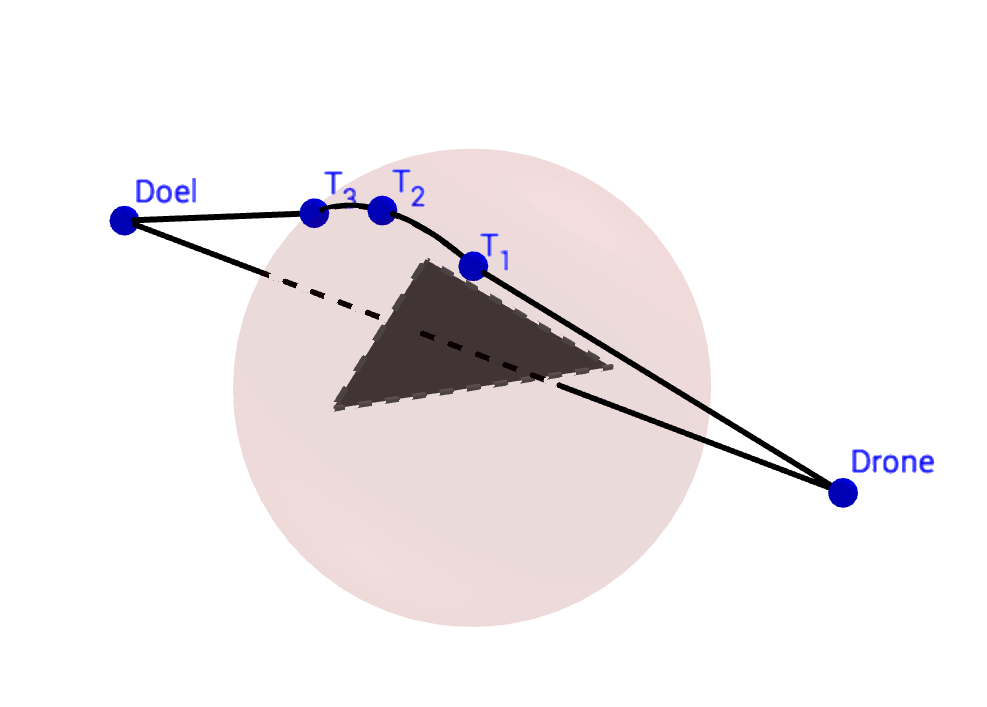
\includegraphics[width=0.6\textwidth]{AP/Obstakel.png}
	\caption{Methode om een obstakel te ontwijken. \(T_1, T_2\) en \(T_3\) stellen tussenstops voor.}
    \label{fig:obstakel}
\end{figure}